\documentclass[tikz,border=3pt]{standalone}
\usepackage[utf8]{inputenc}
\usepackage[T1]{fontenc}
\usepackage{lmodern}
\renewcommand{\familydefault}{\sfdefault}
\usepackage{sansmath}\sansmath
\usepackage{pgfplots}\pgfplotsset{compat=1.18,/pgf/number format/use comma,/pgf/number format/1000 sep={.}}
\usetikzlibrary{arrows.meta,calc,positioning,decorations.pathmorphing,patterns}
% paleta del sitio
\definecolor{nar}{HTML}{E8680C}\definecolor{narc}{HTML}{FFB35C}\definecolor{hielo}{HTML}{FFF3E8}
\definecolor{tinta}{HTML}{1D1D1F}\definecolor{gris}{HTML}{6E6E73}\definecolor{lila}{HTML}{7C5CF0}
\definecolor{azul}{HTML}{2F6FD6}\definecolor{menta}{HTML}{17A673}\definecolor{coral}{HTML}{E8342A}
\begin{document}
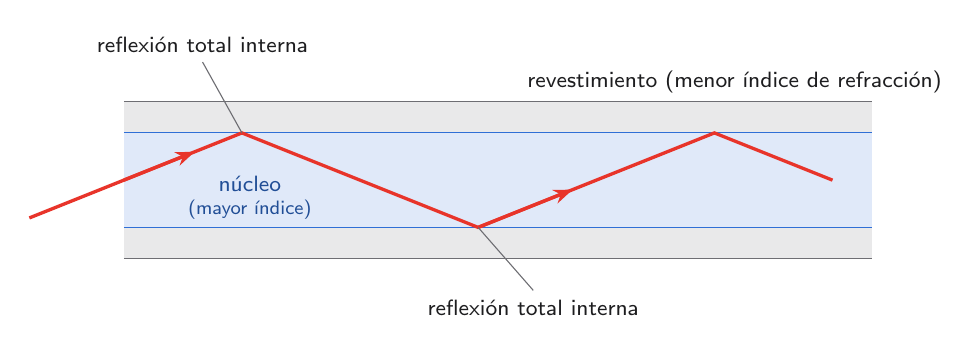
\begin{tikzpicture}[font=\footnotesize,>={Stealth[length=2.4mm]}]
\fill[gris!15] (0,-1.0) rectangle (9.5,1.0);
\fill[azul!15] (0,-0.6) rectangle (9.5,0.6);
\draw[gris] (0,-1.0) -- (9.5,-1.0) (0,1.0) -- (9.5,1.0);
\draw[azul] (0,-0.6) -- (9.5,-0.6) (0,0.6) -- (9.5,0.6);
\draw[very thick,coral] (-1.2,-0.48) -- (0,0) -- (1.5,0.6) -- (4.5,-0.6) -- (7.5,0.6) -- (9,0);
\draw[->,very thick,coral] (0,0) -- (0.9,0.36);
\draw[->,very thick,coral] (4.5,-0.6) -- (5.7,-0.12);
\node[right,text=tinta] at (5.0,1.25) {revestimiento (menor índice de refracción)};
\node[text=azul!70!black] at (1.6,-0.05) {núcleo};
\node[text=azul!70!black,font=\scriptsize] at (1.6,-0.38) {(mayor índice)};
\draw[gris,thin] (1.5,0.6) -- (1.0,1.5) node[above,text=tinta] {reflexión total interna};
\draw[gris,thin] (4.5,-0.6) -- (5.2,-1.4) node[below,text=tinta] {reflexión total interna};
\end{tikzpicture}
\end{document}
